\chapter{Анализ предметной области}

\section{Введение в современные реляционные базы данных}

В мире современной информационной технологии реляционные базы данных играют решающую роль в хранении и управлении информацией, обеспечивая быстрый и структурированный доступ к данным. 
Однако, в многозадачных средах, где множество пользователей одновременно обращается к базам данных, могут возникнуть ситуации, которые представляют серьезные вызовы для обеспечения целостности, производительности и надежности данных. 
Одной из таких ситуаций является взаимная блокировка, или deadlock.

\section{Проблема взаимных блокировок}

В многозадачной среде, где множество пользователей одновременно обращаются к базе данных, возникают ситуации, когда один пользователь ожидает освобождение ресурса (строку или таблицу), необходимый для завершения своей работы, в то время как другой пользователь, в свою очередь ожидает освобождения другого ресурса~\cite{deadlock_defin}. 
Это явление, называемое взаимной блокировкой (deadlock), создает конфликты и приводит к замедлению работы системы. 
Разрешение взаимных блокировок и управление уровнями изоляции становятся ключевыми аспектами обеспечения целостности, производительности и надежности баз данных в таких многопользовательских средах.

\clearpage

На рисунке~\ref{fig:deadlock} приведен пример взаимной блокировки (deadlock)~\cite{deadlock}.
\FloatBarrier
\begin{figure}[h]
	\centering{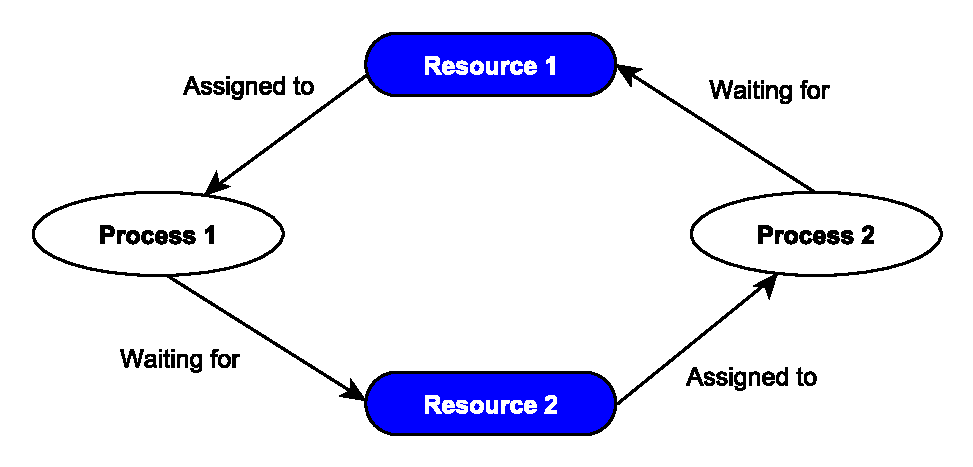
\includegraphics[scale=1]{photos/deadlock.pdf}}
	\caption{Пример взаимной блокировки (deadlock).}
	\label{fig:deadlock}
\end{figure}

Целостность баз данных означает, что данные остаются согласованными и корректными в течение всего их жизненного цикла, несмотря на разнообразные операции и изменения. 

Производительность баз данных связана с способностью обеспечивать высокую скорость доступа к данным и эффективную обработку запросов пользователей.

Надежность баз данных означает, что система сохраняет работоспособность и доступность даже в случае сбоев или непредвиденных ситуаций.

\section{Многопользовательские среды: вызовы и задачи}

Многопользовательская среда представляет собой ситуацию, в которой множество пользователей одновременно взаимодействует с базой данных. 
Это может быть организация, предоставляющая доступ к своей базе данных через сеть, веб-приложение с множеством одновременных пользователей или любая другая среда, где данные используются и изменяются сразу несколькими пользователями. 
В таких средах обеспечение целостности, производительности и надежности баз данных становится особенно актуальным и сложным заданием.

Однако, в контексте многопользовательских сред, возникают уникальные проблемы, связанные с параллельным доступом к данным и управлением транзакциями. 

Транзакция -- совокупность операций, выполняемых прикладной программой, которые переводят согласованное состояние базы данных в согласованное~\cite{transaction}, если:

\begin{itemize}
	\item отсутствуют помехи со стороны других приложений;
	\item транзакция выполнена полностью.
\end{itemize}

\sloppy

Недостаточная координация между пользователями и некорректное управление транзакциями может привести к взаимным блокировкам и конфликтам, которые влияют на целостность данных и производительность системы. 
В таких условиях возникает необходимость в разработке и применении методов обнаружения и разрешения взаимных блокировок.

\clearpage

\section{Взаимоблокировка в многозадачных\\средах}

Наиболее распространенная форма взаимоблокировки возникает, когда два или более потоков ожидают ресурса, который принадлежит другому потоку~\cite{deadlock_detection}. 
Это проиллюстрировано следующим образом:
\FloatBarrier
\begin{table}[h]
	\renewcommand{\arraystretch}{1.8}
	\renewcommand{\tabcolsep}{0.1cm} 
	\begin{center}
		\begin{tabular}{|c|c|} 
			\hline
			Поток1 & Поток2 \\
			\hline
			Принимает блокировку A & Принимает блокировку B \\
			\hline 
			Блокировка запросов B & Запросы блокируют A \\
			\hline
		\end{tabular}
	\end{center}
\end{table}
\FloatBarrier

Если обе последовательности выполняются одновременно, поток 1 никогда не получит блокировку B, так как она принадлежит потоку 2, а поток 2 никогда не получит блокировку A, так как принадлежит потоку 1. 
В лучшем случае это приводит к остановке участвующих потоков, а в худшем~-- к остановке системы.
Реляционная база данных может следить за тем, какие транзакции блокируют какие ресурсы и какие запросы на разблокировку они выполняют.

\clearpage

\chapter{Обзор существующих методов блокировок}

\section{Классификация блокировок}

По области действия блокировки классифицируются на строчные, табличные и предикатные.
По строгости блокировки разделяются на совместные (англ. \textit{shared}) и исключительные (англ. \textit{exclusive}).
По логике реализации блокировки делятся на оптимистические и пессимистические.

В данной теме рассмотрены блокировки базы данных: строчная блокировка, страничная блокировка, блокировка намерений, и табличная блокировка~\cite{data_block}.

\subsection{Строчная блокировка}

Строчная блокировка --- действуют только на одну строку таблицы базы данных, не ограничивая манипуляции над другими строками таблицы.
Снимаются такие блокировки в конце транзакции или при откате к точке сохранения.

Различные СУБД предоставляют разные уровни блокировок на уровне строки, обеспечивая различные уровни изоляции и поведения при параллельном доступе к данным. 
В PostgreSQL, как и во многих других СУБД, существуют различные уровни изоляции транзакций, которые определяют, какие типы блокировок применяются при доступе к строкам данных.

Полный перечень конфликтов блокировок на уровне строк приведён в таблице~\ref{fig:tab-row}. 

\begin{threeparttable}
	\caption{Таблица с режимами блокировки}
	\label{fig:tab-row}
	\begin{tabular}{|c|c|c|c|c|}
		\hline
		\multirow{2}{*}{\textbf{Запрашиваемый}} & \multicolumn{4}{c|}{\textbf{Текущий режим блокировки}} \\
		\cline{2-5} 
		\multirow{2}{*}{\textbf{режим блокировки}}
		& FOR & FOR SHARE & FOR NO KEY & FOR \\
		& KEY & SHARE & UPDATE & UPDATE \\
		\hline
		\textit{FOR KEY SHARE} & & & & X \\
		\hline 
		\textit{FOR SHARE} & & & X & X\\
		\hline
		\textit{FOR NO KEY} & & X & X & X\\
		\textit{UPDATE} & & & &\\
		\hline
		\text{FOR UPDATE} & X & X & X & X \\
		\hline 
	\end{tabular}
\end{threeparttable}
\newline

Можно заметить, что одна транзакция может владеть несколькими конфликтующими блокировками одной строки, даже в разных подтранзакциях; но две разных транзакции никогда не получат конфликтующие блокировки одной и той же строки.

\subsubsection*{FOR UPDATE}

\sloppy

\textit{FOR UPDATE} -- в этом режиме строки, выданные оператором \textit{SELECT}, блокируются как для изменения. 
При этом они защищаются от блокировки, изменения и удаления другими транзакциями до завершения текущей.
То есть другие транзакции, пытающиеся выполнить $UPDATE$, $DELETE$, \textit{SELECT FOR UPDATE}, \textit{SELECT FOR NO KEY UPDATE}, \textit{SELECT FOR SHARE} или \textit{FOR KEY SHARE} с этими строками, будут заблокированы до завершения текущей транзакции.

\subsubsection*{FOR NO KEY UPDATE}

Действует подобно \textit{FOR UPDATE}, но запрашиваемая в этом режиме блокировка слабее: она не будет блокировать команды \textit{SELEСT FOR KEY SHARE}, пытающиеся получить блокировку тех же строк.
Также запрашивается любой командой \textit{UPDATE}, которая не требует блокировки \textit{FOR UPDATE}.

\subsubsection*{FOR SHARE}

Действует подобно \textit{FOR NO KEY UPDATE}, за исключением того, что для каждой из полученных строк запрашивается разделяемая, а не исключительная блокировка. Разделяемая блокировка не позволяет другим транзакциям выполнять с этими строками \textit{UPDATE, DELETE, SELECT FOR UPDATE} или \textit{SELECT FOR NO KEY UPDATE}, но допускает \textit{SELECT FOR SHARE} и \textit{SELECT FOR KEY SHARE}.

\subsubsection*{FOR KEY SHARE}

Действует подобно \textit{FOR SHARE}, но устанавливает более слабую блокировку: блокируется \textit{SELECT FOR UPDATE}, но не \textit{SELECT FOR NO KEY UPDATE}.
Блокировка разделяемого ключа не позволяет другим транзакциям выполнять команды \textit{DELETE} и \textit{UPDATE}, только если они меняют значение ключа (но не другие UPDATE), и при этом допускает выполнение команд \textit{SELECT FOR NO KEY UPDATE}, \textit{SELECT FOR SHARE} и \textit{SELECT FOR KEY SHARE}.

\subsection{Табличная блокировка}

Табличная блокировка (\textit{гранулярная}) --- действует на всю таблицу или всю страницу и все строки.
Блокировка, ограничивающая манипуляции со страницей данных в таблице.

В PostgreSQL существуют различные режимы блокировок, применяемые на уровне таблицы. 
Несмотря на то, что названия некоторых режимов могут казаться связанными с отдельными строками данных, фактически эти режимы применяются ко всей таблице. 
Каждый режим блокировки имеет определенные характеристики и контексты применения, определяемые конфликтующими режимами.

Единственное, что действительно отличает один режим блокировки от другого, это набор режимов, с которыми конфликтует каждый из них.
Конфликтующие блокировки на уровне таблицы можно посмотреть в таблице~\ref{fig:tab-column1}. Две транзакции не могут одновременно владеть блокировками конфликтующих режимов для одной и той же таблицы.

\FloatBarrier
\begin{table}
	\resizebox{\textwidth}{!}{
		\begin{threeparttable}
			\caption{Конфликтующие блокировки на уровне таблицы}
			\label{fig:tab-column1}
			\small
			\begin{tabular}{|c|c|c|c|c|c|c|c|c|}
				\hline
				\multirow{2}{*}{\textbf{Запрашиваемый}} & \multicolumn{8}{c|}{\textbf{Текущий режим блокировки}} \\
				\cline{2-9} 
				\multirow{2}{*}{\textbf{режим}}
				& ACCESS & ROW & ROW & SHARE & & SHARE & & ACCESS \\
				\multirow{2}{*}{\textbf{блокировки}} & SHARE & SHARE & EXCLUSIVE & UPDATE & SHARE & ROW & EXCLUSIVE & EXCLUSIVE \\
				& & & & EXCLUSIVE & & EXCLUSIVE & & \\
				\hline
				\textit{ACCESS} & & & & & & & & X\\
				\textit{SHARE} & & & & & & & & \\
				\hline 
				\textit{ROW} & & & & & & & X & X\\
				\textit{SHARE} & & & & & & & & \\
				\hline
				\textit{ROW }& & & & & X & X & X & X \\
				\textit{EXCLUSIVE} & & & & & & & & \\
				\hline
				\textit{SHARE} & & & & & & & & \\
				\textit{UPDATE} & & & & X & X & X & X & X \\
				\textit{EXCLUSIVE} & & & & & & & & \\
				\hline
				\text{SHARE} & & & X & X & & X & X & X \\
				\hline 
				\textit{SHARE ROW} & & & & & & & & \\
				\textit{ROW} & & & X & X & X & X & X & X \\
				\textit{EXCLUSIVE} & & & & & & & & \\
				\hline
				\textit{EXCLUSIVE} & & X & X & X & X & X & X & X \\
				\hline
				\textit{ACCESS} & X & X & X & X & X & X & X & X \\
				\textit{EXCLUSIVE} & & & & & & & & \\
				\hline
			\end{tabular}
		\end{threeparttable}
	}
\end{table}
\FloatBarrier

Представлены основные режимы блокировок на уровне таблицы.

\subsubsection*{ACCESS SHARE}

Конфликтует только с режимом блокировки \textit{ACCESS EXCLUSIVE}.

Команда \textit{SELECT} получает такую блокировку для таблиц, на которые она ссылается. В ообщем, блокировку в этом режиме получает любой запрос, который только читает таблицу, но не меняет её данные.

\subsubsection*{ROW SHARE}

Конфликтует с режимами блокировки:

\begin{itemize}
	\item EXCLUSIVE;
	\item ACCESS  EXCLUSIVE.
\end{itemize}

Команды \textit{SELECT FOR UPDATE} и \textit{ SELECT FOR SHARE} получают такую блокировку для своих целевых таблиц.

\subsubsection*{ROW EXCLUSIVE}

Конфликтует с режимами блокировки:

\begin{itemize}
	\item SHARE;
	\item SHARE ROW EXCLUSIVE;
	\item EXCLUSIVE;
	\item ACCESS EXCLUSIVE.
\end{itemize}

Команды \textit{UPDATE, DELETE} и \textit{INSERT} получают такую блокировку для целевой таблицы. В ообщем, блокировку в этом режиме получает любая команда, которая изменяет данные в таблице.

\subsubsection*{SHARE UPDATE EXCLUSIVE}

Конфликтует с режимами блокировки:

\begin{itemize}
	\item SHARE UPDATE EXCLUSIVE;
	\item SHARE;
	\item SHARE ROW EXCLUSIVE;
	\item EXCLUSIVE;
	\item ACCESS EXCLUSIVE.
\end{itemize}

Этот режим защищает таблицу от параллельного изменения схемы и запуска процесса~\textit{VACUUM}.

Запрашивается командами:

\begin{itemize}
	\item VACUUM;
	\item ANALYZE;
	\item CREATE INDEX CONCURRENTLY;
	\item CREATE STATISTICS;
	\item COMMENT ON.
\end{itemize}

Также запрашивает \textit{ALTER TABLE VALIDATE} и другими видами \textit{ALTER TABLE}.

\subsubsection*{SHARE}

Конфликтует с режимами блокировки:

\begin{itemize}
	\item ROW EXCLUSIVE;
	\item SHARE UPDATE EXCLUSIVE;
	\item SHARE ROW EXCLUSIVE;
	\item EXCLUSIVE;
	\item ACCESS EXCLUSIVE.
\end{itemize}

Этот режим защищает таблицу от параллельного изменения данных.

Запрашивается командой \textit{CREATE INDEX}.

\subsubsection*{SHARE ROW EXCLUSIVE}

Конфликтует с режимами блокировки:

\begin{itemize}
	\item ROW EXCLUSIVE;
	\item SHARE UPDATE EXCLUSIVE;
	\item SHARE ROW EXCLUSIVE;
	\item EXCLUSIVE;
	\item ACCESS EXCLUSIVE.
\end{itemize}

Этот режим защищает таблицу от параллельных изменений данных и при этом он является самоисключающим, так что такую блокировку может получить только один сеанс.

Запрашивается командой~\textit{CREATE COLLATION},~\textit{CREATE TRIGGER} и многими формами~\textit{ALTER TABLE}.

\subsubsection*{EXCLUSIVE}

Конфликтует с режимами блокировки:

\begin{itemize}
	\item ROW SHARE;
	\item ROW  EXCLUSIVE;
	\item SHARE UPDATE EXCLUSIVE;
	\item SHARE;
	\item SHARE ROW EXCLUSIVE;
	\item EXCLUSIVE;
	\item ACCESS EXCLUSIVE.
\end{itemize}

Этот режим совместим только с блокировкой~\textit{ACCESS SHARE}, то есть параллельно с транзакцией, получившей блокировку в этом режиме, при этом, допускается только чтение таблицы.

Запрашивается командой~\textit{REFRESH MATERIALIZED VIEW\\CONCURRENTLY}.

\subsubsection*{ACCESS EXCLUSIVE}

Конфликтует с режимами блокировок:

\begin{itemize}
	\item ACCESS SHARE;
	\item ROW SHARE;
	\item ROW  EXCLUSIVE;
	\item SHARE UPDATE EXCLUSIVE;
	\item SHARE;
	\item SHARE ROW EXCLUSIVE;
	\item EXCLUSIVE;
	\item ACCESS EXCLUSIVE.
\end{itemize}

Этот режим гарантирует, что кроме транзакции, получившей эту блокировку, никакая другая транзакция не может обращаться к таблице каким-либо способом.

Запрашивается командами \textit{DROP TABLE, TRUNCATE, REINDEX},  \textit{CLUSTER, VACUUM FULL} и \textit{REFRESH MATERIALIZED VIEW}. Блокировку на этом уровне запрашивают также многие виды \textit{ALTER TABLE}. 
В этом режиме по умолчанию запрашивают блокировку, и операторы \textit{LOCK TABLE}, если не был выбран другой режим.

\subsection{Блокировка намерений}

Блокировки намерений, также известные как блокировки намерений для обновления, указывают на намерение изменить определенную строку~\cite{intent_block}.
Блокировки намерений приобретаются, когда транзакция:

\begin{itemize}
	\item выполняет операцию FETCH FOR UPDATE;
	\item выполняет операцию SELECT...FOR UPDATE BY LOCK;
	\item использует \text{SQL\_CONCUR\_LOCK} в качестве основы конкурентности в приложении ODBC (устанавливается с помощью параметра \text{SQL\_ATTR\_CONCURRENCY} вызова API ODBC SQLSetStmtAttr).
\end{itemize}

Блокировки намерений не конфликтуют с блокировками чтения, поэтому приобретение блокировки намерений не блокирует другие транзакции от чтения той же строки. 
Однако блокировки намерений предотвращают другие транзакции от приобретения как блокировки намерений, так и блокировки записи для той же строки, гарантируя, что строка не может быть изменена другой транзакцией перед обновлением.

Если транзакция, выполняющаяся в изоляции снимка, запрашивает блокировку намерений, блокировка намерений приобретается только в том случае, если строка является неизмененной строкой в базе данных и общей для всех одновременных транзакций. 
Однако, если строка является копией снимка, блокировка намерений не приобретается, поскольку исходная строка уже была изменена другой транзакцией. 
Любая попытка снимковой транзакции обновить эту строку завершится неудачей, и будет возвращена ошибка конфликта обновления снимка.

\subsection{Страничная блокировка}

Блокировка данных на уровне страницы подразумевает блокировку группы записей, обычно содержащихся в одной странице базы данных.

Блокировка на уровне страницы может быть полезной в ситуациях, когда несколько транзакций могут одновременно читать и модифицировать разные записи в пределах одной страницы. 
Однако, это также может привести к проблемам с производительностью, таким как <<эффект фантомных записей>>.

Эффект фантомных записей (англ. "phantom read") является одним из аномальных видов чтения данных в многозадачных системах баз данных, где одна транзакция видит изменения, внесенные другой транзакцией, после того как она начала свое выполнение.

Когда транзакция читает ряд данных, который соответствует какому-то условию, и в процессе выполнения другая транзакция добавляет или удаляет записи, соответствующие этому условию, то транзакция, выполняющая чтение, может <<увидеть>> новые записи или не увидеть удаленные записи, что создает впечатление существования <<фантомных>> (воображаемых) записей.

Пример: Транзакция A выполняет запрос SELECT * FROM Orders WHERE Status = 'Новый'; и получает результат.
Транзакция B добавляет новый заказ с Status = 'Новый';.
Транзакция A выполняет тот же запрос снова и видит новый заказ, который был добавлен транзакцией B (фантомный эффект).

Эффект фантомных записей может вызвать проблемы согласованности данных в многозадачной среде. Решения включают в себя использование различных уровней изоляции транзакций, таких как SERIALIZABLE, для предотвращения таких конфликтов.

\subsection{Взаимоблокировка в многозадачных\\средах: детекция и методы разрешения}

После обнаружения взаимных блокировок, система должна разрешить их чтобы продолжить выполнение транзакций. 
Описаны несколько методов разрешения блокировок, такие как:

\begin{itemize}
	\item автоматическое разрешение: СУБД может автоматически определить какую из блокировок следует откатить, чтобы разрешить конфликт и продолжить выполнение транзакцией;
	\item ручное разрешение: администратор базы данных может вмешаться и вручную откатить определенную транзакцию, чтобы разрешить блокировку.
\end{itemize}

Для ручного управления блокировками в реляционных базах данных существует механизм уровня изоляции, который присваивается нужной транзакции и выдает при её работе соответствующие блокировки\cite{isolation}.

Виды уровни изоляции:
\begin{itemize}
	\item Read Uncommitted;
	\item Read Committed;
	\item Snapshot;
	\item Repeatable Read;
	\item Serializable.
\end{itemize}

Read Uncommitted -- полное отсутствие исключительных и разделяемых блокировок. Максимальная производительность работы с такими данными, которые могут быть изменены любой транзакцией и вызвать недействительное чтение.

Read Committed -- разделяемые блокировки присутствуют, пока считываются данные. 

Snapshot -- с данных, к которым обращается транзакция, берется копия. Каждая транзакция может делать это повторно и работать только со своей копией данных.

Repeatable Read -- разделяемые блокировки накладываются на все данные, с которыми работает транзакция.

Serializable -- блокировки диапазона данных с которыми работает транзакция. Во время такой блокировки запрещены вставки и обновления записей другими пользователями.

\section*{Вывод}

Блокировки баз данных играют важную роль в обеспечении целостности данных при параллельном доступе нескольких пользователей или приложений к общим данным.
Они помогают предотвратить конфликты доступа к данным и поддерживают целостность информации.

Блокировка данных ограничивает возможность другим пользователям или приложениям получать доступ или изменять данные во время выполнения операций обновления или изменения. 
Однако использование блокировок на уровне таблицы может снизить производительность приложения из-за ограничения доступа ко всей таблице.

Понимание типов блокировок и их контекстов использования важно для эффективного управления доступом к данным и поддержания целостности базы данных в многопользовательской среде.

